\documentclass[12pt,a4paper]{article}

\usepackage[T1]{fontenc}
\usepackage[utf8]{inputenc} % Use UTF-8 encoding for input
\usepackage[french]{babel}

\usepackage{lmodern}	
\usepackage{amsmath}
\usepackage{amsfonts}
\usepackage{amssymb}
\usepackage{graphicx}
\usepackage{xcolor}
\usepackage{mathtools}
\usepackage{fancyhdr}
\usepackage{enumitem}
\usepackage{tcolorbox}
\usepackage{colortbl}
\usepackage{multirow}
\usepackage{stmaryrd}
\usepackage{dsfont}
\usepackage{tikz}
\usepackage{hyperref}
\usepackage{subcaption}
\usepackage[upgreek]{txgreeks}
\usepackage{algpseudocode}
\usepackage{algorithm}
\usepackage[text={15cm,24.5cm},centering]{geometry}


% Définir le texte affiché en fin de page
\pagestyle{fancy}
\fancyhf{}  % Clear the default headers and footers
\rfoot{\hrule
    \vspace{0.3cm}
    \noindent\textsf{Résolution de systèmes linéaires issus d'EDP}
    \hfill \thepage
}
\renewcommand{\headrulewidth}{0pt}

\title{\vspace{4cm}
        Rapport \\
        \vspace{1cm} \textbf{TP3 : Méthodes Multigrilles} \\ 
        \vspace{4cm} 
}

\author{\textit{Réalisé par} \vspace{0.5cm}\\
         \textbf{Mathilde Ferreira} \\
        \textbf{Félix Foucher de Brandois}
}
        
\date{\vfill
        \textit{ENSEEIHT} - 
        \textit{Formation ModIA, 5$^{e}$ année}
        \hfill
        \textit{2024-2025} \\
        \vspace{1cm}
}


\begin{document}

\begin{figure}[t]
    \centering
    
\includegraphics[width=7cm]{src/inp_n7.png}
    \hfill
    
\includegraphics[width=5.5cm]{src/insa_toulouse.png}
\end{figure}


\maketitle
\thispagestyle{empty}

\newpage


\section{Introduction}

L'objectif de ce TP était d'implémenter une méthode multigrilles en 1D pour résoudre le problème de Poisson avec des conditions aux limites de Dirichlet homogènes.
Le problème est défini par l'équation différentielle suivante :
\begin{equation}
    \begin{cases}
        -u''(x) = f(x) & \text{sur } \Omega = [0,1] \\
        u(0) = u(1) = 0
    \end{cases}
\end{equation}

Pour la discrétisation, nous utilisons une solution exacte connue : $u(x) = x(1-x)$, ce qui donne $f(x) = 2$.
La solution exacte satisfait naturellement les conditions aux limites.

\section{Implémentation et Résultats}

\subsection{Maillage et Discrétisation}

Nous avons discrétisé le problème de Poisson 1D sur un intervalle $[0,1]$ avec un maillage uniforme de $N$ éléments.
La matrice du système linéaire $A$ a été générée à l'aide de la fonction \texttt{getMatrixA(N)}, qui utilise une approximation par différences finies centrées :
$$
A = \frac{1}{h^2} \begin{pmatrix}
    2 & -1 & 0 & \cdots & 0 \\
    -1 & 2 & -1 & \cdots & 0 \\
    0 & -1 & 2 & \cdots & 0 \\
    \vdots & \vdots & \vdots & \ddots & \vdots \\
    0 & 0 & 0 & \cdots & 2
\end{pmatrix} \qquad \text{avec } h = \frac{1}{N}, \text{ la taille de l'intervalle}
$$

\subsection{Lisseur : Méthode de Jacobi Pondérée}

Nous avons utilisé la méthode de Jacobi pondérée pour le lissage, définie par :
\begin{equation}
    \mathbf{u}^{(m+1)} = (I - \omega D^{-1}A)\mathbf{u}^{(m)} + \omega D^{-1}\mathbf{f}
\end{equation}

où $D$ est la matrice diagonale de $A$ et $\omega$ est le paramètre de relaxation.

\subsubsection{Étude du paramètre de relaxation \texorpdfstring{$\omega$}{omega}}

Nous avons analysé l'effet du paramètre $\omega$ sur la convergence pour le mode $k=6$ :

\begin{figure}[H]
    \centering
    \begin{subfigure}{0.45\textwidth}
        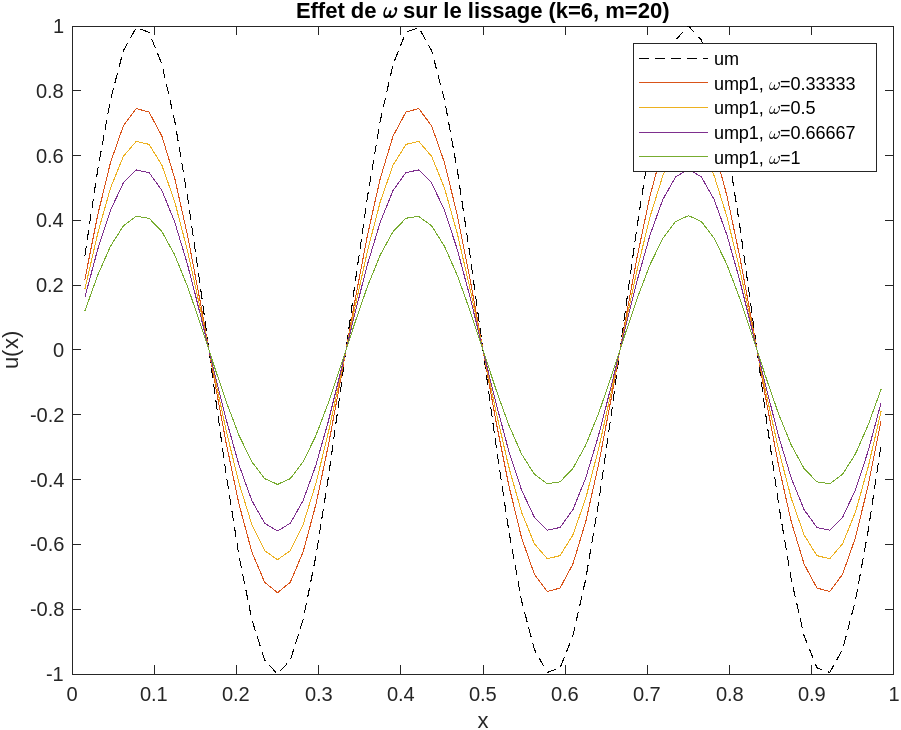
\includegraphics[width=\textwidth]{src/omega.png}
        \caption{Convergence en fonction de $\omega$.}
        \label{fig:omega_convergence}
    \end{subfigure}
    \hfill
    \begin{subfigure}{0.45\textwidth}
        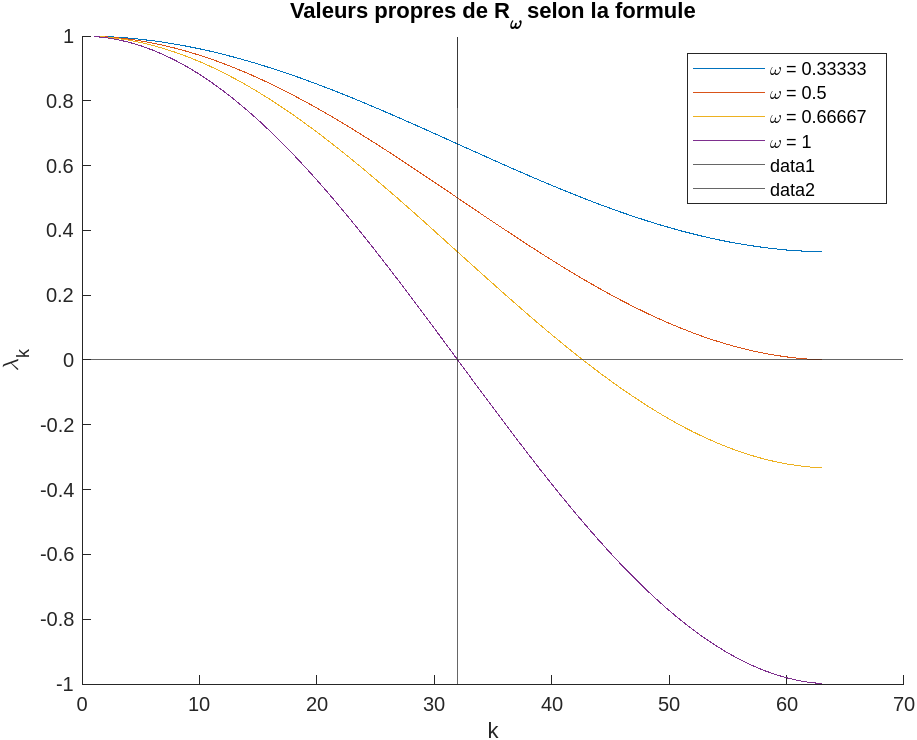
\includegraphics[width=\textwidth]{src/lambda_k.png}
        \caption{Valeurs propres $\lambda_k(R_\omega)$ pour différents $\omega$.}
        \label{fig:lambda_k}
    \end{subfigure}
    \caption{Analyse de l'effet du paramètre $\omega$.}
    \label{fig:omega_analysis}
\end{figure}

Pour trouver la valeur optimale de $\omega$, on doit chercher la valeur qui minimise l'intervalle $\left[-\bar{\lambda}, \bar{\lambda}\right]$, avec $\lambda_k(R_\omega) \in \left[-\bar{\lambda}, \bar{\lambda}\right]$ pour $\frac{N}{2} \leq k \leq N - 1$.\\

On obtient la valeur optimale $\omega^* = 2/3$.


\subsubsection{Effet du nombre d'itérations}
Nous avons également étudié l'effet du nombre d'itérations de lissage sur la convergence :

\begin{figure}[H]
    \centering
    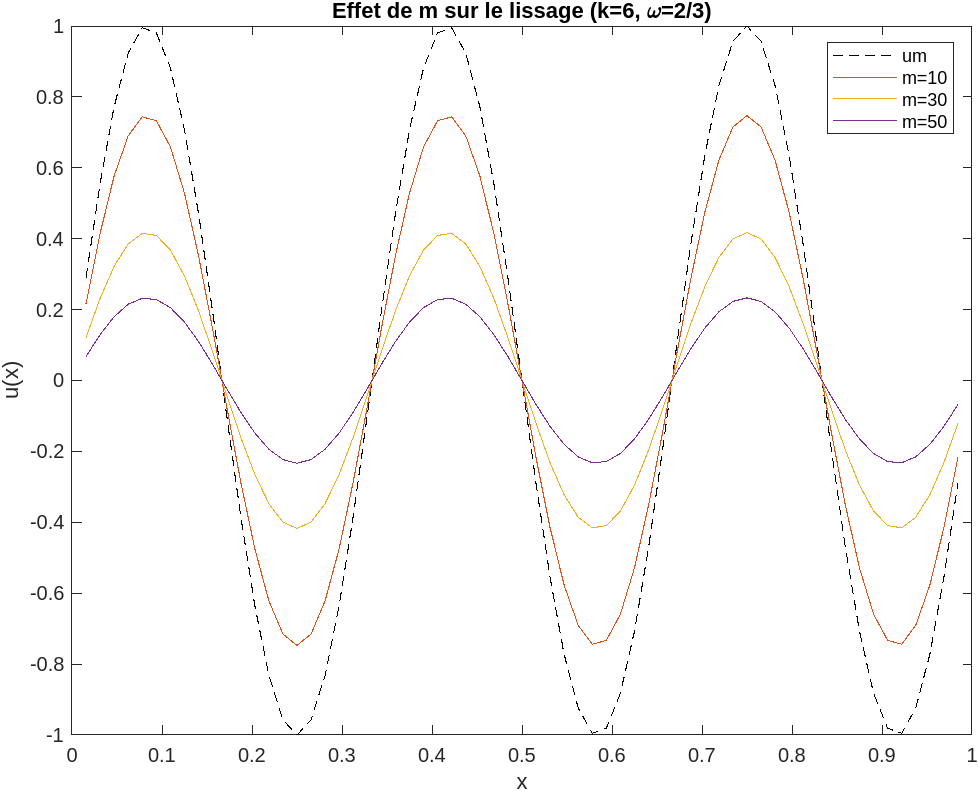
\includegraphics[width=0.7\textwidth]{src/iterations.png}
    \caption{Convergence en fonction du nombre d'itérations de lissage.}
    \label{fig:iterations_convergence}
\end{figure}

Plus le nombre d'itérations est élevé, plus l'erreur diminue.


\subsubsection{Effet du vecteur propre \texorpdfstring{$k$}{k} choisi}

Nous avons étudié l'effet du vecteur propre $k$ sur le lissage

\begin{figure}[H]
    \centering
    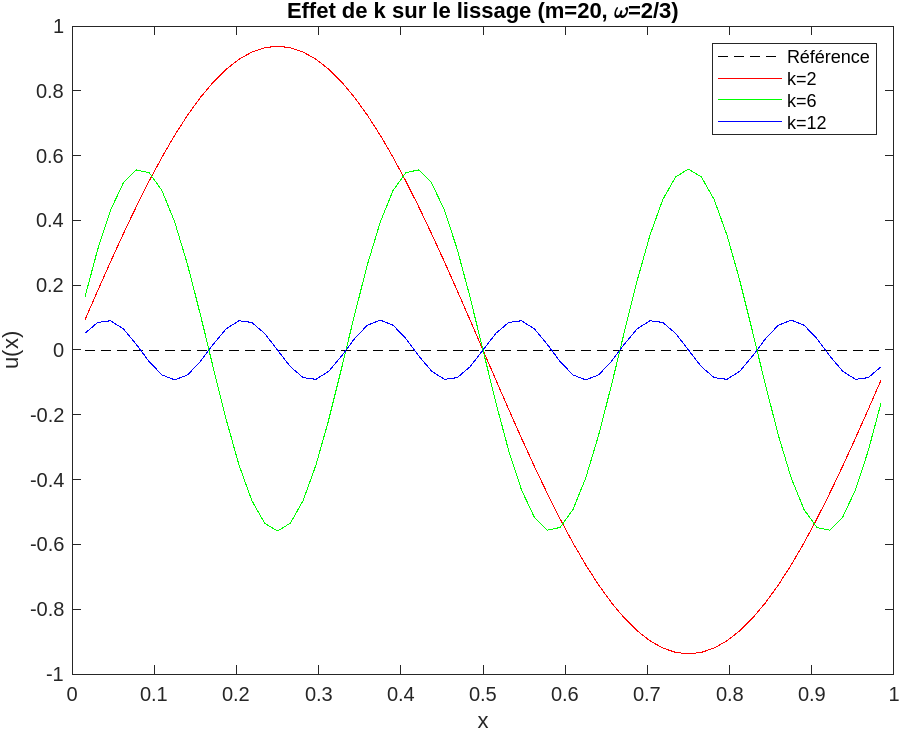
\includegraphics[width=0.6\textwidth]{src/k.png}
    \caption{Convergence en fonction du mode propre $k$.}
    \label{fig:k_convergence}
\end{figure}

On observe que l'erreur est plus amortie pour les grandes valeurs de $k$ (mode oscillatoire) que pour les petites valeurs de $k$ (mode propre).


\subsection{Opérateurs de Transfert}
Pour transférer les informations d’un maillage à l’autre, il nous faut des opérateurs de transfert inter-grilles.
Nous avons utilisé l’interpolation linéaire pour la prolongation et le full-weighting pour la restriction :
\begin{itemize}
    \item Prolongation : $I_{2h}^h = \frac{1}{2}
    \begin{pmatrix}
    1 & 0 \\
    2 & 0 \\
    1 & 1 \\
    0 & 2 \\
    0 & 1 \\
    \end{pmatrix}$
    
    \item Restriction : $I_{h}^{2h} = \frac{1}{2} {I_{2h}^h}^T$
\end{itemize}

L'avantage d'utiliser ce couple d'opérateurs est qu'il permet de n'en implémenter qu'un seul, grâce à la relation entre les deux.

\subsection{Principe Multigrille}

Nous avons implémenté un cycle à deux niveaux avec :
\begin{enumerate}
    \item \textbf{Pré-lissage} : 2 itérations de Jacobi pondérée sur le maillage fin.
    \item \textbf{Correction sur le maillage grossier :}
    \begin{itemize}
        \item Calcul du résidu sur le maillage fin : $r_h = f - A_h v$.
        \item Restriction du résidu sur le maillage grossier : $r_{2h} = I_{h}^{2h} r_h$.
        \item Résolution exacte sur le maillage grossier : $A_{2h} e_{2h} = r_{2h}$.
        \item Prolongation de la correction sur le maillage fin : $e_h = I_{2h}^h e_{2h}$.
        \item Mise à jour de la solution : $v = v + e_h$. \\
    \end{itemize}
\end{enumerate}

Ce schéma permet d'éliminer les erreurs de haute fréquence grâce au lissage, et les erreurs de basse fréquence grâce à la correction sur le maillage grossier.


\subsection{Résultats Numériques}

La méthode multigrilles montre une convergence rapide et indépendante de la taille du maillage, comme le montre la réduction de l'erreur $\|u_\text{ref} - v\|$ après chaque itération :

\begin{figure}[H]
    \centering
    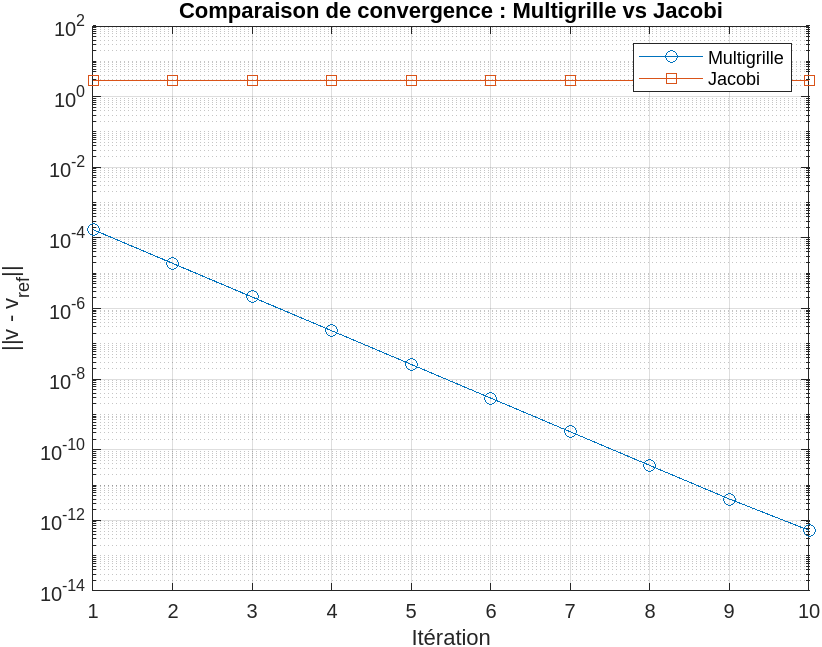
\includegraphics[width=0.7\textwidth]{src/convergence.png}
    \caption{Convergence de la méthode multigrilles.}
    \label{fig:multigrid_convergence}
\end{figure}

On observe que la méthode multigrilles converge vers la solution exacte. \\

Par la suite, nous avons adapté le critère d'arrêt : au lieu de s'arrêter après un nombre fixe d'itérations, on calcule le résidu à chaque étape du processus itératif.
$$
q^{(m)} = \frac{\|res^{(m)}_h \|_ 2}{\|res^{(0)}_h \|_2} = \frac{\|f - A_h v^{(m)} \|_2}{\|f - A_h v^{(0)} \|_2}
$$

Nous avons ensuite étudié l'effet de la taille du maillage sur le nombre d'itérations nécessaires pour atteindre un critère d'arrêt donné ($q^{(m)} < 10^{-10}$) :

\begin{table}[H]
    \centering
    \begin{tabular}{|c|c|}
        \hline
        \rowcolor{gray!20} \textbf{Taille du maillage $N$} & \textbf{Nombre d'itérations} \\
        \hline
        32 & 12 \\
64 & 12 \\
128 & 12 \\
256 & 12 \\
        \hline
    \end{tabular}
    \caption{Temps d'exécution en fonction de la taille du maillage}
    \label{tab:execution_time}
\end{table}

On observe que le nombre d'itérations reste constant : le nombre d'itérations ne dépend pas de la taille du maillage $N$.


\end{document}